\chapter{Graph-Datenbanken und -Frameworks - Ausgewählte Systeme }
\section{PostgreSQL}
\subsection{Allgemein}
    \begin{itemize}
        \item Kategorie / Modell
            \subitem PostgreSQL ist ein Relationales Datenbank System \cite{postgresqldoc}
        \item Version
            \subitem Aktuelle Major Version: 11
        \item Historie
            \subitem PostgreSQL ist aus dem POSTGRES projekt der University of California at Berkeley entstanden, welches unter der Leitung von  Professor Michael Stonebraker im Jahre 1986 began.
            SQL Interpreter seit 1994, das System hieß zu diesem Zeitpunkt Postgres95. 1996 wurde es in PostgrSQL umbenannt.\cite{postgresqldoc}
        \item Hersteller
        \item Lizenz
            \subitem Open-Source

    \end{itemize}
PostgreSQL ist eine Objektrelationale Datenbank. Weiterentwicklungen wird von der PostgreSQL Global Development Group durchgeführt. PostgreSQL steht unter der PostgreSQL-Lizenz, welche sehr stark der GNU-Lizenz ähnelt. Auf Basis von PostgreSQL gibt es mehrere, zum Teil auch kommerzielle, Forks wie zum Beispiel Amazon Redshift oder EnterpriseDB.
\subsection{Architektur}
    \begin{itemize}
        \item Programmiersprache des Systems
        \item Systemkomponenten, Systemarchitektur
        \subitem client / server Architektur \cite{postgresqldoc}
        \item Betriebsart
            \subitem Cluster - Menge an Datenbanken, die von PostSQL-Server verwaltet werden \cite{froehlich01}
        \item Protokoll der Schnittstelle
        \subitem TCP/IP
        \item API
    \end{itemize}
    Die Architektur von PostgresSQL ist in folgendem Bild gegeben:
    \begin{center}
        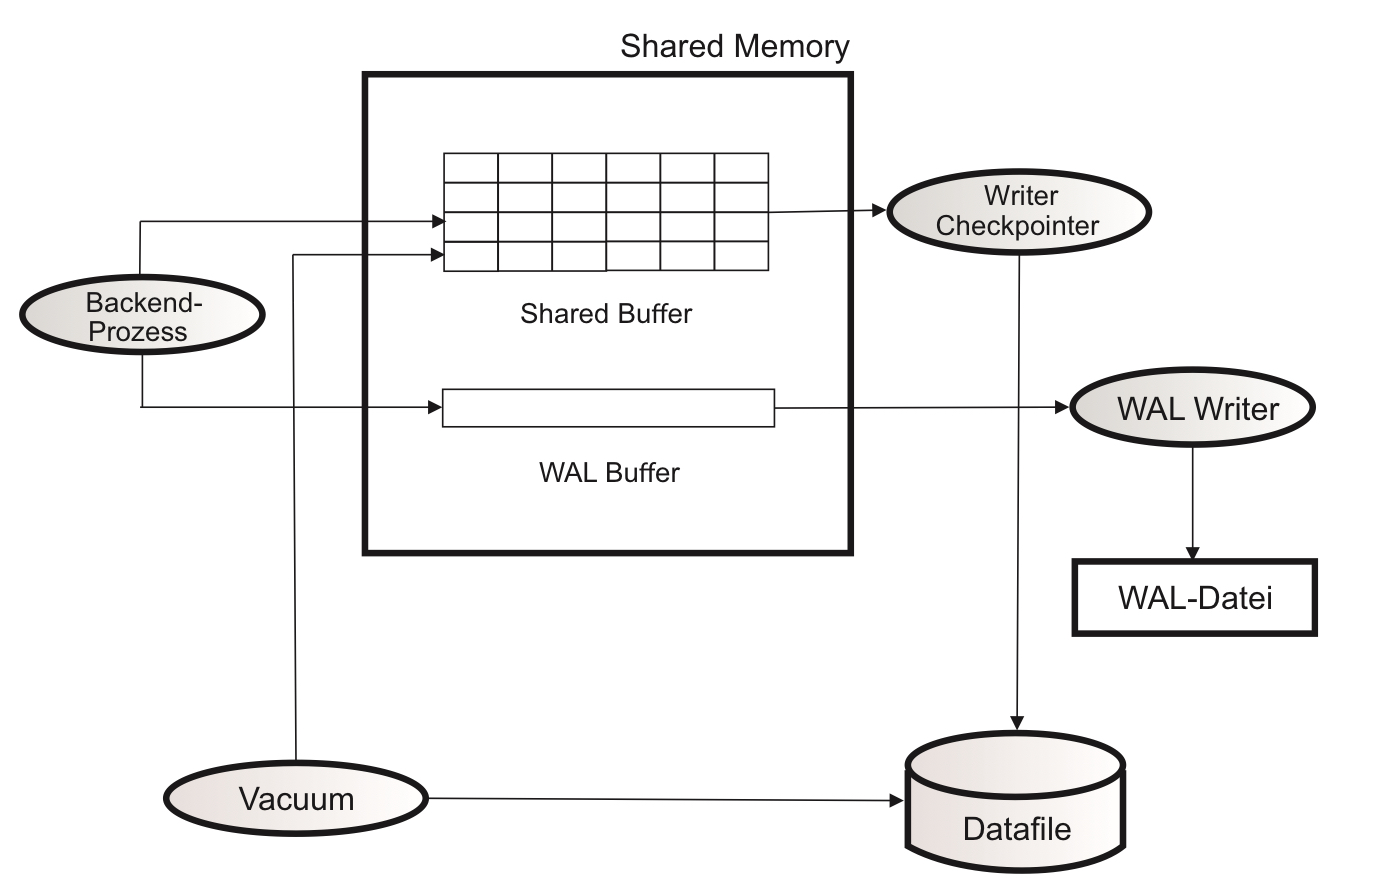
\includegraphics[width = \linewidth]{./images/PostgresSQLArchitektur.jpg}
    \end{center}
    Diese Architektur ergibt sich aus der Gegebenheit, dass alle Daten normalerweise nicht in den Shared Buffer passen. Ein Teil der Datenbank befindet sich im Datafile, aus dem bei Bedarf gelesen werden kann, der andere Teil im Shared Buffer.
    Die Hauptaufgabe des Shared Buffer ist es, Input Output Operationen (I/O Operationen) auf das Datafile zu minimieren und möglichst viele Operationen im Speicher durchzuführen. Die Motivation möglichst viele Operation im Speicher durchzuführen
    besteht darin, dass Operationen im Speicher schneller ausgeführt werden. Werden Operationen im Speicher ausgeführt, so werden I/O Operationen auf das Datafile reduziert. Der Writer Prozess ist für die Synchronisation
    des Zustands des Shared Buffers und der Tablespaces verantwortlich. Dieser Prozess schreibt Datenblöcke aus dem Shared Buffer auf die Tablespaces innerhalb des Datafile. Neben diesem writer Prozess gibt es noch andere BackenProzesse, die in dem Bild unter BackendProzess zusammengefasst sind
    Der Writer Checkpoint ist dafür verantwortlich, dass alle geänderten Datenblöcke innerhalb des Shared Buffer in das Datafile geschrieben werden. Der WAL (Write-Ahead Log) Buffer, der WAL Writer sowie die WAL-Datei bilden das Transaktionslog des Clusters. Sie werden genauer im Kapitel Konsistenz beschrieben.
    \footnote{Vgl. \cite[Seite 26]{froehlich01}} VACUUM beschreibt den Prozess, der Teil der Verwaltung mehrere Versionen
    von Datenbankblöcken ist. In Postgres werden verschiedene Versionen von Datensätzen in der Tabelle gespeichert. Ältere Versionen von den Datensätzen werden gelöscht, wenn sie nicht mehr benötigt werden. Dadurch entstehen
    Lücken in der Tabelle, die der Vacum Prozess als nicht mehr benötigt kennzeichnet. \footnote{Vgl. \cite[Seite 37]{froehlich01}}

    Eine PostgreSQL-Instanz wird als Server Prozess mit eigenem Datenverzeichnis und einer eigenen Konfigurationsdatei sowie einem eigenen Transaktionslog.
\subsection{Datenmodell}
    \begin{itemize}
        \item Standardsprache: SQL
        \item Objektbegriff, Konzepte: Relationale Datenbank - Abbildung in Tabellen
        \item Datentypen:
        \subitem Sehr viele unterstützte Datentypen, es lassen sich aber auch eigene Datentypen mittesl des CREATE TYPE befehls erstellen.\cite{postgres8}
    \end{itemize}
    Daten werden in Form von Tabellen abgelegt. Im Filesystem legt PostgreSQL Dateien im sogenannten \$PGDATA-Verzeichnis ab, dieses wird beim Start von PostgreSQL festgelegt. Alle Date werden im Verzeichnis Base unterhalb von \$PGDATA abgelegt. Einzelne Tabellen oder Indices können in Tablespaces ausgelagert werden. Für einen Tablespace wird ein neuer Unterordner im \$PGDATA-Verzeichnis angelegt. Es ist auch möglich einzelne Spalten einer Tabelle in einen anderen Tablespace zu verschieben.
\subsection{Konsistenz}
PostgreSQL schreibt einen Transaktionslog (Write-Ahead Log, WAL).
Dieser wird als WAL-Buffer im Arbeitsspeicher und als WAL-Dateien auf der Festplatte geführt.
Bei jedem Commit einer Transaktion wird zunächst das WAL aktualisiert bevor die Bestätigung an den Client gesendet wird.
Der walwriter-Prozess schreibt periodisch die WAL-Buffer auf die Festplatte.
\subsection{Indexe}
\subsection{Anfragemethoden}
\subsection{Konsistenz}

